%% Self-contained ICML-format draft. Compiles with plain pdflatex, no
%% icml2027.sty required. Swap in the official style file when released.
\documentclass[10pt,letterpaper,twocolumn]{article}

\usepackage[letterpaper,left=0.9in,right=0.9in,top=1.0in,bottom=1.0in]{geometry}
\setlength{\columnsep}{0.25in}

\usepackage[T1]{fontenc}
\usepackage{times}
\usepackage{microtype}
\usepackage{graphicx}
\usepackage{booktabs}
\usepackage{multirow}
\usepackage{siunitx}
\usepackage[ruled,vlined]{algorithm2e}
\usepackage{amsmath,amssymb,amsthm,mathtools}
\usepackage{bm}
\usepackage{xcolor}
\usepackage{enumitem}
\usepackage{caption}
\usepackage{titlesec}
\usepackage{natbib}
\usepackage[colorlinks=true,linkcolor=black,citecolor=black,urlcolor=blue]{hyperref}

\captionsetup{font=small,labelfont=bf,skip=4pt}
\titleformat{\section}{\normalfont\large\bfseries}{\thesection}{0.6em}{}
\titleformat{\subsection}{\normalfont\normalsize\bfseries}{\thesubsection}{0.6em}{}
\titlespacing*{\section}{0pt}{1.2ex plus .3ex}{0.7ex}
\titlespacing*{\subsection}{0pt}{1.0ex plus .3ex}{0.5ex}

\newcommand{\TODO}[1]{\textcolor{red}{\small\textbf{[TODO:}~\textit{#1}\textbf{]}}}
\newcommand{\GATE}[1]{\textcolor{blue}{\textsf{\scriptsize (#1)}}}
\newcommand{\DONE}[1]{\textcolor{teal}{\small\textbf{[VERIFIED:}~\textit{#1}\textbf{]}}}

\newcommand{\X}{\mathcal{X}}
\newcommand{\Y}{\mathcal{Y}}
\newcommand{\bff}{\mathbf{f}}
\newcommand{\bfg}{\mathbf{g}}
\newcommand{\bfL}{\mathbf{L}}
\newcommand{\bfN}{\mathbf{N}}
\newcommand{\dKL}{d_{\mathrm{KL}}}
\newcommand{\dLLV}{d^{\lambda}_{\mathrm{LLV}}}
\newcommand{\dSVD}{d_{\mathrm{SVD}}}
\newcommand{\dfg}{d_{\bff,\bfg}}
\newcommand{\Dalpha}{D_{\alpha}}
\newcommand{\Dinf}{D_{\infty}}
\newcommand{\psix}{\psi_{x}}
\newcommand{\psiy}{\psi_{y}}
\newcommand{\TV}{\mathrm{TV}}
\newcommand{\Var}{\mathrm{Var}}
\newcommand{\simL}{\sim_{L}}
\newcommand{\Thetadelta}{\Theta_{\delta}}
\newcommand{\Cov}{\mathrm{Cov}}
\newcommand{\mCCA}{m_{\mathrm{CCA}}}

\theoremstyle{plain}
\newtheorem{theorem}{Theorem}
\newtheorem{lemma}[theorem]{Lemma}
\newtheorem{proposition}[theorem]{Proposition}
\newtheorem{corollary}[theorem]{Corollary}
\theoremstyle{definition}
\newtheorem{definition}[theorem]{Definition}
\newtheorem{assumption}[theorem]{Assumption}
\theoremstyle{remark}
\newtheorem{remark}[theorem]{Remark}

\begin{document}

\twocolumn[
\begin{center}
{\LARGE\bfseries Which Divergences Control Representations?\\[2pt]
Tail Sensitivity and the Limits of Identifiability\par}
\vspace{8pt}
{\normalsize Anonymous Author(s)\par}
{\small Anonymous Institution\par}
\vspace{10pt}
\end{center}

\begin{minipage}{\textwidth}
\begin{center}\begin{minipage}{0.86\textwidth}
\begin{abstract}
\small
Identifiability theory says that two models in the softmax family with
\emph{equal} likelihood have representations equal up to an invertible linear
map. Trained models agree only approximately, and it is known that vanishing
Kullback--Leibler divergence does not imply similar representations --- leaving
open which notions of distributional closeness, if any, do. We show the answer
turns on one property. Representational error is an \emph{unweighted} spread of
log-likelihood ratios, and those ratios are largest where probability mass is
smallest, whereas classical divergences weight each label by its own mass. We
call the gap \emph{tail sensitivity} and index it by R\'enyi order $\alpha$.
Exact asymptotics give a critical order $\alpha^{\star}_{\mathrm{sym}}>1$, so
every order $\alpha\le1$ --- total variation, Hellinger, Jensen--Shannon and KL
--- fails outright; a dichotomy shows $\alpha^{\star}_{\mathrm{sym}}=\infty$
only for linearly equivalent pairs, and a graded bound gives similarity at rate
$O(1/\alpha)$ above threshold. Two consequences are practical. KL's guarantee
is unusable for any model, since the $(M{+}1)$-th largest probability is at most
$1/(M{+}1)$; but a sharpened perturbation bound certifies $58\%$ of retrained
CIFAR-10 pairs where the previous constant certified none. We supply a
four-number diagnostic, computable in one forward pass, that bounds in advance
what a likelihood comparison can reveal. On $3{,}800$ synthetic and $705$ CIFAR-10 model pairs spanning four representation dimensions we show that matched
likelihood is least informative exactly when models are confident and
representations wide, and confirm the mechanism causally: rescaling logits
leaves representational dissimilarity invariant to machine precision while
raising the confidence floor nine orders of magnitude, and the association
between likelihood and representation strengthens significantly
($+0.109$, $95\%$ CI $[+0.044,+0.202{]}$).
\end{abstract}
\end{minipage}\end{center}
\vspace{10pt}
\end{minipage}
]


%%%%%%%%%%%%%%%%%%%%%%%%%%%%%%%%%%%%%%%%%%%%%%%%%%%%%%%%%%%%%%%%%%%%%%%%%%%%%%%
\section{Introduction}
\label{sec:intro}

Whether independently trained networks learn related representations is an
active question \citep{kornblith2019,klabunde2025}, and any answer depends on
what counts as ``the same'' representation. Identifiability theory supplies a
principled choice: in the softmax family of Eq.~\eqref{eq:model}, two models
with equal likelihood have embeddings equal up to an invertible linear map
\citep{roeder2021,khemakhem2020icebeem,lachapelle2023}, so a similarity measure
should be invariant to exactly that class.

Exact equality is not what happens. Trained models agree approximately, and
\citet{nielsen2025} showed this is not enough: two models can have vanishing
KL divergence and dissimilar representations. It is tempting to read that as a
fact about KL and look for a better divergence. We argue it is a fact about a
\emph{property} KL lacks, and that naming the property settles the question for
a whole family at once.

\paragraph{Tail sensitivity.}
Write $r_{y}(x)=\log p(y|x)-\log p'(y|x)$. The representational error between
two models is a variance of these log-ratios across labels
(Sec.~\ref{sec:positive}) --- an \emph{unweighted} spread. But $r_{y}$ is
largest exactly where $p(y|x)$ is smallest, while every classical divergence
weights label $y$ by its own mass. A divergence can control representations
only if it stays sensitive to log-ratios at labels carrying vanishing mass. The
R\'enyi order $\alpha$ tunes precisely this weighting, from the mass-weighted
average at $\alpha=1$ to the worst-case ratio at $\alpha=\infty$, so the
question becomes one about position on a single axis.

\paragraph{Contributions.}
\begin{itemize}[leftmargin=1.2em,itemsep=1pt,topsep=2pt]
\item \emph{Control} (Def.~\ref{def:control}), making divergence--representation
      claims falsifiable and uniform over a model class.
\item Exact rate asymptotics and a closed-form critical order
      (Thm.~\ref{thm:alphastar}), verified to solver precision; hence all
      orders $\alpha\le1$ fail (Cor.~\ref{cor:below}).
\item A dichotomy (Thm.~\ref{thm:dichotomy}), graded control
      (Thm.~\ref{thm:graded}) and an explicit finite cap
      (Cor.~\ref{cor:ceiling}), confining the controlling orders to an interval.
\item A perturbation bound improving the known modulus by $\sqrt{M}$
      (Thm.~\ref{thm:maxdiv}), whose non-vacuity is capped by an identity
      (Prop.~\ref{prop:ceiling}) that trained networks nonetheless satisfy: it
      certifies $58\%$ of retrained CIFAR-10 pairs against $0\%$ before.
\item A four-number diagnostic (Alg.~\ref{alg:diag}) and experiments on
      $3{,}800$ synthetic and $270$ CIFAR-10 pairs, including a confound-free
      temperature intervention.
\end{itemize}

%%%%%%%%%%%%%%%%%%%%%%%%%%%%%%%%%%%%%%%%%%%%%%%%%%%%%%%%%%%%%%%%%%%%%%%%%%%%%%%
\section{Setup}
\label{sec:setup}

Models are pairs $(\bff,\bfg)\in\Theta$ with embedding
$\bff:\X\to\mathbb{R}^{M}$ and unembedding $\bfg:\Y\to\mathbb{R}^{M}$:
\begin{equation}
p_{\bff,\bfg}(y\mid x)=\frac{\exp(\bff(x)^{\top}\bfg(y))}
{\sum_{y'\in\Y}\exp(\bff(x)^{\top}\bfg(y'))}.
\label{eq:model}
\end{equation}
Write $\bff_{0}(x)=\bff(x)-\bff(x_{0})$, $\bfg_{0}(y)=\bfg(y)-\bfg(y_{0})$; let
$\bfL$ have columns $\bfg_{0}(y_{i})$ and $\bfN$ columns $\bff_{0}(x_{i})$,
$i=1..M$. Under the \emph{diversity} condition --- that both sets span
$\mathbb{R}^{M}$ --- equal likelihoods force $\bff=\mathbf{A}\bff'$ and
$\bfg_{0}=\mathbf{A}^{-\top}\bfg'_{0}$ for one invertible $\mathbf{A}$; write
$(\bff,\bfg)\simL(\bff',\bfg')$. Diversity is mild where labels are plentiful
($|\Y|\sim10^{4}$ against $M\sim10^{3}$ in language models) but binds for image
classifiers with fewer classes than representation dimensions.

Following \citet{nielsen2025} we measure dissimilarity with $\dfg$, built from
the PLS-SVD statistic $\dSVD$ applied to $\bfL^{\top}\bff(x)$ and
$\bfN^{\top}\bfg(y)$ (Alg.~\ref{alg:dfg}, App.~\ref{app:alg}). It vanishes
exactly on $\simL$-equivalent pairs, and unlike CCA-based measures is not
invariant to every invertible linear map: its invariance class is fixed by the
identifiability result rather than chosen. We compare against $\mCCA$, linear
CKA and Procrustes throughout.

\paragraph{Why this invariance class.}
The choice is not free. CCA-based measures are invariant to \emph{every}
invertible linear map, so they attain their maximum on pairs related by maps
that identifiability does not license, and cannot distinguish
$\simL$-equivalence from a weaker linear relation; CKA restricts to orthogonal
maps and isotropic scaling, which is narrower than $\simL$ in the other
direction. $\dfg$ is invariant to exactly the transformations that leave the
model likelihood unchanged, which is what a measure must respect if
``similar'' is to mean ``indistinguishable from the data''. It also couples
embeddings and unembeddings --- $\bfL$ depends on $\bfg$ and $\bfN$ on $\bff$
--- so it cannot be fooled by a pair whose embeddings match while their
unembeddings do not. We do not claim this is the only defensible choice, and we
report $\mCCA$, CKA and Procrustes alongside it throughout
(Sec.~\ref{sec:exp}); they agree within each representation dimension.

\begin{definition}[Control]
\label{def:control}
A divergence $D$ \emph{controls} $\dfg$ on $\Theta$ if there is a
nondecreasing $h$ with $h(0^{+})=0$ such that for all pairs in $\Theta$,
$D(p_{\bff,\bfg},p_{\bff',\bfg'})\le\epsilon\Rightarrow\dfg\le h(\epsilon)$.
\end{definition}

Control is uniform over $\Theta$; a divergence may fail on $\Theta$ yet control
on a subclass. Since $\Dalpha$ is nondecreasing in $\alpha$, the set of
controlling orders is upward closed, so
$\alpha^{\star}_{\Theta}:=\inf\{\alpha:\Dalpha\text{ controls}\}$ is well posed.
The rest of the paper brackets it.

%%%%%%%%%%%%%%%%%%%%%%%%%%%%%%%%%%%%%%%%%%%%%%%%%%%%%%%%%%%%%%%%%%%%%%%%%%%%%%%
\section{No Order at or below One Controls}
\label{sec:negative}

Fix $x$, write $s_{y}=\cos(\bff(x),\bfg(y))$, $\hat y=\arg\max_{y}s_{y}$, and
let $a_{y}=s_{\hat y}-s_{y}>0$ and $b_{y}=s'_{\hat y}-s'_{y}>0$ be the
\emph{margin gaps} of the two models. Along the norm-growth family of
\citet{nielsen2025} the unembeddings have common norm $\rho$, so logits are
$c\rho s_{y}$ and
\begin{equation}
p(y|x)=\frac{e^{-c\rho a_{y}}}{Z_{\rho}},\qquad
p'(y|x)=\frac{e^{-c\rho b_{y}}}{Z'_{\rho}},
\label{eq:family}
\end{equation}
with $a_{\hat y}=b_{\hat y}=0$. Every off-top term vanishes as $\rho\to\infty$,
so $Z_{\rho},Z'_{\rho}\to1$:

\begin{lemma}[Co-concentration]
\label{lem:coconc}
Both models converge to the \emph{same} point mass,
$p(\hat y|x)\to1$ and $p'(\hat y|x)\to1$, so $\|p-p'\|_{\TV}\to0$; meanwhile
$|r_{y}|=c\rho|b_{y}-a_{y}|+O(1)=\Theta(\rho)$ whenever $a_{y}\neq b_{y}$.
\end{lemma}

This is the mechanism in one line: the two distributions become
indistinguishable in any mass-weighted sense while their log-ratios diverge.
Whether a divergence notices depends on how it weights the tail. Define the
\emph{tilted exponent} $E_{\alpha}(y)=\alpha a_{y}+(1-\alpha)b_{y}
=b_{y}+\alpha(a_{y}-b_{y})$, which governs the R\'enyi integrand
$p^{\alpha}p'^{1-\alpha}\propto e^{-c\rho E_{\alpha}(y)}$.

\begin{theorem}[Rate lemma and critical order]
\label{thm:alphastar}
Let
\begin{equation}
\alpha^{\star}=\min_{y\,:\,b_{y}>a_{y}}\frac{b_{y}}{b_{y}-a_{y}} .
\label{eq:alphastar}
\end{equation}
Then $\alpha^{\star}>1$, and as $\rho\to\infty$: \emph{(i)} for
$\alpha<\alpha^{\star}$, $\Dalpha=\Theta(e^{-c\rho\kappa(\alpha)})$, where
$\kappa$ is the smallest exponent in
$\{E_{\alpha}(y)\}\cup\{a_{y}\}\cup\{b_{y}\}$ carrying a non-vanishing
coefficient; \emph{(ii)} at $\alpha=1$ all first-order coefficients cancel and
$\dKL=\Theta(\rho\,e^{-c\rho a_{\min}})$; \emph{(iii)} for
$\alpha>\alpha^{\star}$, $\Dalpha$ grows \emph{linearly} in $\rho$ with slope
$\max_{y}(-E_{\alpha}(y))/(\alpha-1)$.
\end{theorem}

\begin{proof}[Sketch]
Expanding $\log\sum_{y}p^{\alpha}p'^{1-\alpha}$ to first order and grouping the
three exponent families by value, the coefficient at value $v$ is
$\#\{E_{\alpha}=v\}-\alpha\#\{a=v\}+(\alpha-1)\#\{b=v\}$. A label with
$a_{y}=b_{y}$ has $E_{\alpha}(y)=a_{y}=b_{y}$ and contributes
$1-\alpha+(\alpha-1)=0$: such labels \emph{cancel exactly} and must be excluded,
which is the one non-obvious step. At $\alpha=1$ every coefficient vanishes,
forcing the second-order term and its polynomial prefactor. Finally
$E_{\alpha}$ is affine in $\alpha$ with $E_{0}(y)=b_{y}>0$, decreasing only
when $a_{y}<b_{y}$, and vanishing at $b_{y}/(b_{y}-a_{y})$; since
$0<b_{y}-a_{y}<b_{y}$, that value exceeds $1$. Full proof in
App.~\ref{app:neg}.
\end{proof}

\begin{table}[t]
\centering\small
\caption{Rate lemma against exact computation, single input, $k=7$,
$\rho\le160$. The lemma is per-direction and verifies in both:
$\alpha^{\star}_{\mathrm{fwd}}=1.349915$ (bisected $1.349919$) and
$\alpha^{\star}_{\mathrm{rev}}=1.276277$ (bisected $1.276430$), so
$\alpha^{\star}_{\mathrm{sym}}=1.2763$.}
\label{tab:rate}
\begin{tabular}{@{}lllr@{}}
\toprule
$\alpha$ & branch & predicted & measured \\
\midrule
$0.5$      & exp    & $0.2866$ & $0.2866$ \\
$1.0$ (KL) & exp    & $0.2866$ & $0.2866$ \\
$1.1$      & exp    & $0.2047$ & $0.2044$ \\
$1.3$      & exp    & $0.0409$ & $0.0401$ \\
$1.6$      & linear & $0.3414$ & $0.3414$ \\
$2.0$      & linear & $0.5325$ & $0.5324$ \\
$\infty$   & linear & $0.8623$ & $0.8623$ \\
\bottomrule
\end{tabular}
\end{table}

That $\alpha^{\star}>1$ is the whole negative result:

\begin{corollary}
\label{cor:below}
Total variation, squared Hellinger, Jensen--Shannon and Kullback--Leibler all
fail to control $\dfg$. The known KL counterexample is the boundary case
$\alpha=1$ of a one-parameter statement.
\end{corollary}

\begin{figure*}[t]
\centering
\includegraphics[width=0.92\textwidth]{fig_ladder.pdf}
\caption{\textbf{(a)} Divergence ladder along the norm-growth family of
Eq.~\eqref{eq:family}. Every order $\alpha\le1$, KL included, decays toward
zero; orders above $\alpha^{\star}$ grow linearly in $\rho$, as
Thm.~\ref{thm:alphastar}(iii) predicts. The faint horizontal lines are $\dfg$,
$\mCCA$ and $\dLLV$: the representations do not move at all, so every decaying
curve is a divergence losing sight of a difference that is still there.
\textbf{(b)} Predicted against measured exponential decay rate over $739$
(geometry, order) pairs spanning $2.3$ decades; median relative error $2.3\%$.
This is the panel that exercises the cancellation rule of
Thm.~\ref{thm:alphastar}(i) --- labels with $a_{y}=b_{y}$ must be excluded, and
omitting them inflates predicted rates by $40$--$70\%$. \textbf{(c)}
$\alpha^{\star}_{m}$, the critical order restricted to inputs whose margin
exceeds $m$, for three label counts. Without conditioning, $\alpha^{\star}$ is
pinned just above $1$ by whichever single input lies nearest a decision
boundary: bisectors have codimension one, so any full-dimensional input support
crosses them. The threshold is a property of the worst-margin input, not of the
representational geometry.}
\label{fig:ladder}
\end{figure*}

Verification is exact (Tab.~\ref{tab:rate}): across $295$ geometries the
median relative error in the crossover is $0.00\%$, decay rates match to
$<2.3\%$ and growth slopes to $<0.1\%$. Omitting the cancellation rule inflates
predicted rates by $40$--$70\%$.

\begin{theorem}[Uniform separation]
\label{thm:lower}
Along the norm-growth family $\dSVD$ is \emph{exactly} independent of $\rho$,
so any non-$\simL$-equivalent pair stays separated by a constant $c>0$ of the
geometry alone.
\end{theorem}

\begin{remark}[Averaging preserves the rate, not the constant]
\label{rem:avg}
Thm.~\ref{thm:alphastar} is per-input. Averaging over an input distribution
leaves the decay exponential rather than turning it into a power law
($R^{2}=1.00$ against $0.91$ for a power-law fit), but the rate is set by the
\emph{minimum} margin in the support: it falls from $0.193$ to $0.018$ when
clusters are allowed to touch the decision boundary. Rates should therefore be
quoted against a margin floor, which is what Fig.~\ref{fig:ladder}(c) does.
\end{remark}

\begin{remark}[Both directions]
\label{rem:asym}
R\'enyi divergence is asymmetric, so the meaningful quantity is
$\alpha^{\star}_{\mathrm{sym}}=\min\{\alpha^{\star}(p\|p'),\alpha^{\star}(p'\|p)\}$:
a family is a counterexample only if both directions stay small. Computing only
the forward direction reports $\infty$ whenever $b_{y}\le a_{y}$ for every $y$,
even though the reverse divergence then diverges.
\end{remark}

%%%%%%%%%%%%%%%%%%%%%%%%%%%%%%%%%%%%%%%%%%%%%%%%%%%%%%%%%%%%%%%%%%%%%%%%%%%%%%%
\section{What Does Control, and How Far}
\label{sec:positive}

Everything positive follows from one perturbation bound. With
$z_{1}=\bfL^{\top}\bff(x)$, $z_{2}=\bfL'^{\top}\bff'(x)$ and
$\Delta_{l}=z_{1,l}-z_{2,l}=r_{y_{l}}-r_{y_{0}}$, set
$\mathrm{sd}_{l}=\operatorname{std}(\Delta_{l})$,
$\tau_{l}=|s_{l}-s'_{l}|$ and $\psi_{l}=\min(s_{l},s'_{l})$, where
$s_{l},s'_{l}$ are the coordinate standard deviations. Note
$s_{l}=\psix(y_{l};p)$, the non-degeneracy already present in the LLV
construction.

\begin{theorem}[Perturbation bound]
\label{thm:maxdiv}
Let $\lambda_{\max}=\lambda_{\max}(\mathrm{Corr}(z_{1}))\le M$. Then
\begin{equation}
\dfg\ \le\ \sqrt{\lambda_{\max}}\,Q,\qquad
Q^{2}=\frac1M\sum_{l}\Big(\frac{\tau_{l}+\mathrm{sd}_{l}}{\psi_{l}}\Big)^{2}.
\label{eq:maxdiv-bound}
\end{equation}
In particular $\Dinf\le\epsilon$ gives
$\dfg\le4\sqrt{\lambda_{\max}}\,\epsilon/\psi_{\min}$.
\end{theorem}

Two steps are new relative to a naive estimate, and both are free
(App.~\ref{app:pos}). Hoffman--Wielandt replaces a per-singular-value Weyl
bound, saving $\sqrt{M}$:
\begin{proposition}[Tighter spectral step]
\label{prop:tighten}
$\sum_{i}(\sigma_{i}-\tilde\sigma_{i})^{2}\le\|E\|_{F}^{2}$ and
Cauchy--Schwarz give
$\dSVD\le(\sum_{l}\Var[z'_{l}-w'_{l}])^{1/2}$, improving the known
$(M\sum_{l}\Var)^{1/2}$ by $\sqrt{M}$.
\end{proposition}
Second, $\tau_{l}$ is kept
separate from $\mathrm{sd}_{l}$ rather than bounded by it, which is wasteful
because the difference of standard deviations is much smaller than the standard
deviation of the difference (median $\tau_{l}/\mathrm{sd}_{l}$ is
$0.25$--$0.53$). Jointly they tighten the bound by $1.65$--$2.37\times$, and on
CIFAR-10 by $1.67\times$ --- the difference between certifying nothing and
certifying a majority (Sec.~\ref{sec:exp}).

\begin{theorem}[KL on $\Thetadelta$]
\label{thm:klcond}
Let $\Y_{m}\subseteq\Y$ satisfy diversity with $|\Y_{m}|\ge M+1$, take
$\mathcal{Y}_{\mathrm{LLV}}\subseteq\Y_{m}$ and
$\delta_{m}=\min_{x}\min_{y\in\Y_{m}}\min\{p,p'\}$. If $\dKL\le\epsilon$ then
$\dfg\le4\sqrt{2\lambda_{\max}\epsilon}/(\delta_{m}\psi_{\min})$.
\label{eq:klbound}
\end{theorem}

\begin{theorem}[Dichotomy]
\label{thm:dichotomy}
Under diversity,
$\alpha^{\star}_{\mathrm{sym}}=\infty\iff p_{\bff,\bfg}=p_{\bff',\bfg'}
\iff(\bff,\bfg)\simL(\bff',\bfg')$.
Every non-equivalent pair therefore has a \emph{finite} critical order.
\end{theorem}

\begin{proof}[Sketch]
Both directions infinite forces $a_{y}(x)=b_{y}(x)$ for all $x,y$. Writing
$R_{y}(x)=\bff(x)^{\top}\bfg(y)-\bff'(x)^{\top}\bfg'(y)$ and using
$a_{y}-b_{y}=R_{\hat y}-R_{y}$, this says $R_{y}(x)=c(x)$ is independent of
$y$; an additive $c(x)$ cancels in the softmax normaliser, so the conditionals
coincide and linear identifiability applies. The converse is immediate.
\end{proof}

A regression test over $329$ pairs gives
$\max|\dfg|=5.0\times10^{-4}$ in the infinite class against
$\min|\dfg|=6.5\times10^{-2}$ in the finite class, the residual decaying as
$O(1/n)$.

\begin{theorem}[Graded control]
\label{thm:graded}
With $\Delta=\sup_{x,y}a_{y}(x)$, if $\alpha^{\star}_{\mathrm{sym}}\ge A$ then
$\dfg\le4\sqrt{M}\Delta/(\psi_{\min}A)=O(1/A)$.
\end{theorem}

\begin{proof}[Sketch of Thm.~\ref{thm:graded}]
$\alpha^{\star}_{\mathrm{sym}}\ge A$ gives
$|a_{y}-b_{y}|\le\max(a_{y},b_{y})/A\le\Delta/A$; since
$a_{y}-b_{y}=R_{\hat y}-R_{y}$, the map $y\mapsto R_{y}(x)$ lies within
$\Delta/A$ of a constant, so $|\Delta_{l}|\le2\Delta/A$. Apply
Thm.~\ref{thm:maxdiv}.
\end{proof}

\DONE{Thm.~\ref{thm:graded} is violated on $0/435$ trained CIFAR-10 pairs
and $0/45$ at $M{=}8$ (previously checked only on $67$ constructed
geometries), but it is loose: the bound exceeds the realised $\dfg$ by a median
$623\times$ at $M{=}2$ and $1286\times$ at $M{=}8$. Cor.~\ref{cor:ceiling} below is algebraically the same inequality
rearranged and inherits both the validity and the slack.}

\begin{corollary}[The ceiling is finite]
\label{cor:ceiling}
For any $d_{0}>0$,
$\alpha_{0}(d_{0}):=\sup\{\alpha^{\star}_{\mathrm{sym}}:\dfg\ge d_{0}\}
\le4\sqrt{M}\Delta/(\psi_{\min}d_{0})<\infty$.
\end{corollary}

Together: $\alpha^{\star}_{\mathrm{sym}}>1$ from below,
$\alpha^{\star}_{\mathrm{sym}}<\infty$ from above, and an explicit cap between.
Searches over permutation classes, dimensions, norm profiles and angular
arrangements place the empirical ceiling at $1.35$ (App.~\ref{app:extra}).

\subsection{What can and cannot be certified}
\label{sec:cannot}

The three obstructions are not alike.

\textbf{(i)} Orders $\alpha\le1$ fail qualitatively (Cor.~\ref{cor:below}); no
constant repairs them.

\textbf{(ii)} Thm.~\ref{thm:klcond} is non-vacuous only for
$\epsilon<\delta_{m}^{2}/64$, and the floor cannot be lifted:
\begin{proposition}[KL's floor is capped]
\label{prop:floorcap}
For any model $\delta_{M+1}\le1/(M+1)$, since $M+1$ entries each exceeding it
would sum to more than one. Hence \eqref{eq:klbound} is below $1$ only for
$\epsilon<1/(64(M+1)^{2})$; at $M=2$ this is $\epsilon<1.7\times10^{-3}$.
\end{proposition}
On CIFAR-10 the realised requirement is
$\epsilon<1.2\times10^{-31}$ against observed KL of order one. Quantile floors do not help: discarding the worst
$10\%$ of inputs buys nine orders and leaves thirteen. This is tail
insensitivity written as an inequality --- $\dKL$ is a mass-weighted average of
log-ratios while $\rho_{2}$ is their unweighted spread, and conversion pays the
ratio of the two measures.

\begin{corollary}[Confidence, not quality]
\label{cor:conf}
Two models can have arbitrarily small $\dKL$ and arbitrarily large $\dfg$
precisely when $\delta_{m}$ is small. Since accurate classifiers and language
models place negligible mass on most labels, these are exactly the regimes in
which likelihood agreement carries least representational information ---
raising $\delta_{m}$ should therefore make the association between $\dKL$ and
$\dfg$ either stronger or at least detectable.
\end{corollary}

\textbf{(iii)} By contrast, the sup-log-ratio route \emph{does} certify.
\begin{proposition}[Non-vacuity is capped]
\label{prop:ceiling}
$\sum_{l}\Var[z'_{l}-w'_{l}]\ge2M\dSVD$ by trace $\le$ nuclear norm, so
$\mathrm{bound}\ge\sqrt{2\lambda_{\max}\dSVD}$ and $\mathrm{bound}<1$ forces
$\dfg<1/(2\lambda_{\max})\le\frac12$.
\end{proposition}
Whether that cap binds is empirical, and on CIFAR-10 it does not:
$\lambda_{\max}=1.44$--$3.46$ over $M=2,3,5$ gives ceilings $0.347$--$0.145$
against median $\dfg$ of $0.128$, $0.065$, $0.103$. So of the three
obstructions only two are real; the third was a technique gap.

\subsection{A diagnostic instead of a certificate}
\label{sec:diagnostic}

\begin{algorithm}[t]
\caption{Critical order $\alpha^{\star}_{\mathrm{sym}}$}
\label{alg:astar}
\SetAlgoLined
\KwIn{$\log p,\log p'$ on $N$ inputs; margin floor $m\ge0$}
\KwOut{$\alpha^{\star}_{\mathrm{sym}}$; $=\infty$ iff $p=p'$
       (Thm.~\ref{thm:dichotomy})}
$\hat y\leftarrow\arg\max_{y}\log p$;\ \ $\hat y'\leftarrow\arg\max_{y}\log p'$\;
keep inputs with $\hat y=\hat y'$ and $\min_{y\neq\hat y}a_{y}\ge m$;
\textbf{report} the retained fraction\;
$\alpha_{\rightarrow}\leftarrow\min\{b_{y}/(b_{y}-a_{y}):b_{y}>a_{y}\}$\;
$\alpha_{\leftarrow}\leftarrow\min\{a_{y}/(a_{y}-b_{y}):a_{y}>b_{y}\}$\;
\Return $\min(\alpha_{\rightarrow},\alpha_{\leftarrow})$
  \tcp*{both: Rem.~\ref{rem:asym}}
\end{algorithm}

\begin{algorithm}[t]
\caption{Pre-comparison diagnostic}
\label{alg:diag}
\SetAlgoLined
\KwIn{two trained models; held-out inputs}
\KwOut{what any likelihood comparison between them can reveal}
$\delta_{M+1}\leftarrow\min_{x}\,(M{+}1)$-th largest $p(y|x)$\;
\lIf{observed $\dKL>\delta_{M+1}^{2}/64$}{\textbf{KL cannot certify}}
$\lambda_{\max}\leftarrow\lambda_{\max}(\mathrm{Corr}(z_{1}))$;\quad
\textbf{ceiling} $\leftarrow1/(2\lambda_{\max})$\;
$Q^{2}\leftarrow\frac1M\sum_{l}((\tau_{l}+\mathrm{sd}_{l})/\psi_{l})^{2}$;\quad
\textbf{bound} $\leftarrow\sqrt{\lambda_{\max}}Q$\;
\lIf{bound $<1$}{\textbf{certified}: $\dfg\le$ bound}
$\alpha^{\star}_{\mathrm{sym}}\leftarrow$ Alg.~\ref{alg:astar}
  \tcp*{order at which the pair becomes visible}
\end{algorithm}

\begin{table}[t]
\centering\small
\caption{The diagnostic applied to a pair of retrained CIFAR-10 models
($M=2$). Four numbers, one forward pass, read before any similarity claim.}
\label{tab:diag}
\begin{tabular}{@{}llp{3.0cm}@{}}
\toprule
quantity & value & what it says \\
\midrule
$\delta_{M+1}$ & $1.1\!\times\!10^{-15}$ &
  KL is informative only below $\epsilon\!\approx\!10^{-31}$; observed
  $\dKL\!=\!0.60$, so KL certifies nothing \\
$\lambda_{\max}$ & $1.442$ &
  ceiling $1/(2\lambda_{\max})=0.347$; pairs above this can never be certified \\
bound & $0.931$ &
  below $1$, so the pair is certified; the observed $\dfg$ is well inside it \\
$\Delta/\psi_{\min}$ & $11.3$ &
  Cor.~\ref{cor:ceiling} would need $\alpha>64$, far above the threshold
  near $1.35$ \\
\bottomrule
\end{tabular}
\end{table}

Four quantities, one forward pass, bounding in advance what a likelihood
comparison can reveal. Tab.~\ref{tab:diag} works through a real pair. $\delta_{M+1}$ says whether KL can say anything;
$\lambda_{\max}$ fixes the largest dissimilarity the method could ever rule
out, and grows with $M$, so the certificate is a low-dimensional instrument;
$\Delta/\psi_{\min}$ sets the order Cor.~\ref{cor:ceiling} would require; and
$\alpha^{\star}_{\mathrm{sym}}$ says where on the R\'enyi scale the pair
becomes distinguishable, being infinite exactly when the models are equivalent.

\subsection{Open problem: how large is $\alpha_{0}$?}
\label{sec:open}

Thm.~\ref{thm:alphastar} and Thm.~\ref{thm:dichotomy} confine the controlling
orders to $(1,\alpha_{0}{]}$, and Cor.~\ref{cor:ceiling} turns any bound on
$\alpha_{0}$ into a control modulus. What remains open is whether
$\alpha_{0}<\infty$ \emph{uniformly}, without fixing a dissimilarity level.

All our searches place it near $1.3$ (Tab.~\ref{tab:mscale}). Exhaustively over
the $720$ permutations at $k=6$, order-breaking pairs reach $1.09$ and
reflections $1.11$; a factorial over input concentration, angular regularity,
norm profile and dimension tops out at $1.20$; a targeted search over
reflection-composed permutations ($921$ configurations) reaches $1.14$. Two
structural facts explain the ceiling. First,
$\alpha^{\star}_{\mathrm{sym}}\!\to\!1$ whenever an input approaches a decision
boundary of one model while the other ranks the tied labels differently, and
bisectors have codimension one. Second, at $M=2$ the unembeddings carry a
cyclic order, and an order-breaking permutation cannot be realised without a
collision: the census shows $\alpha^{\star}_{\mathrm{sym}}=\infty$ exactly on
the rotations, which are globally linear and have $\dfg=0$, while every
order-breaking permutation is pinned near $1.05$ however dissimilar its
representations. The obstruction is topological, not metric --- flat in the
number of order violations and unmoved by non-uniform norms.

\begin{table}[t]
\centering\small
\caption{$\alpha^{\star}_{\mathrm{sym}}$ saturates in representation dimension.
Margin floor $0.08$, $\dfg\ge0.10$ required, $200$ random geometries per $M$;
$n$ survives both filters. Medians sit at $1.00$: almost every non-equivalent
pair has a critical order barely above $1$.}
\label{tab:mscale}
\begin{tabular}{@{}lrrrrrr@{}}
\toprule
$M$ & 2 & 3 & 4 & 6 & 8 & 12 \\
\midrule
$n$                                  & 144 & 199 & 192 & 182 & 177 & 183 \\
best $\alpha^{\star}_{\mathrm{sym}}$ & 1.34 & 1.31 & 1.20 & 1.26 & 1.18 & 1.22 \\
median                               & 1.004 & 1.002 & 1.001 & 1.001 & 1.002 & 1.002 \\
$\dfg$ at best                       & 0.12 & 0.33 & 0.32 & 0.42 & 0.24 & 0.41 \\
\bottomrule
\end{tabular}
\end{table}

%%%%%%%%%%%%%%%%%%%%%%%%%%%%%%%%%%%%%%%%%%%%%%%%%%%%%%%%%%%%%%%%%%%%%%%%%%%%%%%
\section{Experiments}
\label{sec:exp}

Full protocols, sample sizes and negative controls are in
App.~\ref{app:exp}--\ref{app:extra}. Rank correlations carry $95\%$ cluster
bootstrap intervals over \emph{seeds}: $n$ seeds give $\binom{n}{2}$ dependent
pairs, so pair-level resampling is anticonservative. No pair was dropped and no
bound was violated anywhere.

\paragraph{Guards.}
The analysis reports rather than silently drops: the count of discarded pairs
(zero everywhere), the per-pair argmax agreement (median $0.804$ on CIFAR-10,
minimum $0.607$), and the assertion
$\alpha^{\star}_{\mathrm{sym}}=\infty\Rightarrow\dfg<5/n$ implied by
Thm.~\ref{thm:dichotomy}, whose tolerance is $5/n$ because the residual is
$O(1/n)$ estimator bias rather than noise. These are released as a test suite;
three substantive errors during this work were silent filters, and we recommend
reading the guard lines before the results.

\paragraph{Synthetic: wider networks learn closer distributions and more
dissimilar representations.}
$400$ models ($c\in\{4,6,10,18\}$ classes, widths $16$--$256$, $20$ seeds,
$15$k steps), $3{,}800$ pairs. Mean training loss is flat in width
($0.0202\to0.0208$ at $c{=}4$), so width and fit quality are separated. In that
regime mean $\dKL$ \emph{falls} with width ($5.06\to1.65$ at $c{=}10$) while
mean $\dfg$ \emph{rises} ($0.436\to0.697$); loss-adjusted regression leaves the
slope positive in all four class counts ($+0.034$ to $+0.098$). The effect is
not an artefact of our invariance class: under $\mCCA$, the measure used in
prior width studies, similarity falls monotonically with width in every class
count ($0.741\to0.666$ at $c{=}4$; $0.639\to0.530$ at $c{=}6$), after applying
the $\ge90\%$ accuracy filter of \citet{roeder2021}. Applying that filter removes $1{,}080$ of $3{,}800$ pairs but leaves the trend
untouched where it is applied evenly: filtered means agree with the unfiltered
ones to three decimals at $c{=}4,6,10$ (e.g.\ $0.4345\to0.6969$ against
$0.436\to0.697$ at $c{=}10$). We rest the claim on $c{=}4$ and $c{=}6$, where
the filter removes essentially nothing; the $c{=}18$ cells retain as few as
three pairs and are uninformative (App.~\ref{app:extra}). This is the paper's thesis made visible
on trained models at scale, and it is consistent with recent reports that
convergence trends under CKA are confounded by width and depth
\citep{aristotelian2026,platoscave2026,structure2026}. We vary hidden width at
fixed $M$ and fixed dataset size, so the result speaks only to that slice.

\paragraph{Control curves.}
Tab.~\ref{tab:control} reports the empirical modulus
$\hat h(\epsilon)=\sup\{\dfg:D\le\epsilon\}$ --- the direct counterpart of
Def.~\ref{def:control} --- at quantiles of each divergence. All divergences
show substantial empirical control on \emph{trained} models, with the higher
orders falling further ($\hat h$ ratio $0.075$ at $\alpha\ge1.5$ against
$0.113$ for KL and $0.313$ for total variation, the least tail-sensitive). The
ordering matches the theory but the effect is weak: over $2{,}720$ pairs
surviving the accuracy filter, $\dKL$ still tracks $\dfg$ at
$\rho=0.602$ ($95\%$ cluster bootstrap over seeds $[0.506,0.705]$), so the
worst case our constructions realise is not generic under training. We regard this as
delimiting the theory rather than undermining it.



\paragraph{CIFAR-10: a temperature intervention isolates the mechanism.}
Sixty ResNet18 \citep{he2016} models on CIFAR-10 \citep{krizhevsky2009},
$M\in\{2,3,5,8\}$, ten seeds each plus a smoothing arm, and a $30$-seed arm
at $M{=}2$ for the temperature study; $705$ pairs in total. Rescaling
logits by $1/T$ leaves $\dfg$ \emph{exactly} invariant, since $\dSVD$
standardises its inputs, while $\delta_{3}$ rises: this holds representational
dissimilarity fixed and moves only the confidence floor. Two things are then
facts rather than inferences (Tab.~\ref{tab:temp}): $\delta_{3}$ climbs nine
orders of magnitude, and mean $\dfg$ stays at $0.1918$ with maximum change
$0.00$.

The rank correlation between $\dKL$ and $\dfg$ then rises monotonically across
all five temperatures, $0.652\to0.761$. Because the same pairs appear at every
$T$, the claim is about the \emph{change} in $\rho$, and a paired cluster
bootstrap over seeds gives $\rho(T{=}16)-\rho(T{=}1)=+0.109$ with $95\%$
interval $[+0.044,+0.202]$ and $P(\text{increase})=0.9998$. Raising the
confidence floor strengthens the association between likelihood agreement and
representational agreement, with representational dissimilarity held exactly
fixed --- which is Cor.~\ref{cor:conf} in its stronger form.

We note that this required $30$ seeds. At $10$ the same experiment gave
$+0.090$ with interval $[-0.049,+0.395]$: the effect was present but not
establishable, because the binding resource is the number of independent
training runs, not the number of temperatures. The dimensional comparison of
Tab.~\ref{tab:c3} retains $10$ seeds per dimension so that $M{=}2,3,5$ stay
balanced.


\begin{table}[t]
\centering\small
\caption{Temperature sweep, CIFAR-10, $435$ pairs from $30$ seeds. Rescaling
logits leaves $\dfg$ invariant to machine precision, so only the confidence
floor moves. Intervals are $95\%$ cluster bootstrap over seeds. A paired
bootstrap on the same pairs puts $\rho(T{=}16)-\rho(T{=}1)$ at $+0.109$ with
interval $[+0.044,+0.202]$, so the rise is significant.}
\label{tab:temp}
\begin{tabular}{@{}lrrrl@{}}
\toprule
$T$ & $\delta_{3}$ & mean $\dKL$ & $\dfg$ & $\rho$ \,[95\% CI] \\
\midrule
$1$  & $7.9\!\times\!10^{-11}$ & 0.601 & 0.1918 & 0.652 \,$[0.37,0.80]$ \\
$2$  & $8.5\!\times\!10^{-6}$  & 0.409 & 0.1918 & 0.689 \,$[0.42,0.83]$ \\
$4$  & $2.5\!\times\!10^{-3}$  & 0.289 & 0.1918 & 0.714 \,$[0.46,0.85]$ \\
$8$  & $3.5\!\times\!10^{-2}$  & 0.183 & 0.1918 & 0.736 \,$[0.50,0.86]$ \\
$16$ & $9.6\!\times\!10^{-2}$  & 0.096 & 0.1918 & \textbf{0.761} \,$[0.54,0.88]$ \\
\bottomrule
\end{tabular}
\end{table}

\begin{table}[t]
\centering\small
\caption{Empirical modulus $\hat h(\epsilon)$ on $3{,}800$ trained synthetic
pairs, at quantiles of each divergence. Last column is
$\hat h(q_{.05})/\hat h(q_{.5})$; smaller means the modulus falls faster as
$\epsilon\to0$, i.e.\ closer to control.}
\label{tab:control}
\begin{tabular}{@{}lrrrr@{}}
\toprule
 & $q_{.05}$ & $q_{.25}$ & $q_{.5}$ & ratio \\
\midrule
Total variation   & 0.259 & 0.750 & 0.827 & 0.313 \\
R\'enyi $0.5$     & 0.093 & 0.827 & 0.827 & 0.113 \\
KL ($\alpha{=}1$) & 0.093 & 0.633 & 0.827 & 0.113 \\
R\'enyi $1.5$     & 0.056 & 0.633 & 0.750 & \textbf{0.075} \\
R\'enyi $2$       & 0.072 & 0.633 & 0.750 & 0.096 \\
R\'enyi $\infty$  & 0.072 & 0.673 & 0.949 & \textbf{0.075} \\
\bottomrule
\end{tabular}
\end{table}

\begin{table}[t]
\centering\small
\caption{Mean $\mCCA$ against hidden width, after the $\ge90\%$ accuracy filter
of \citet{roeder2021} ($315/400$ models kept). $\mCCA$ is a \emph{similarity},
so a falling row is rising dissimilarity. The $c{=}18$ block is reported for
completeness only: the filter removes models so unevenly there that its cells
compare differently-selected subpopulations.}
\label{tab:mcca}
\begin{tabular}{@{}l rrrrr@{}}
\toprule
 & \multicolumn{5}{c}{hidden width $w$} \\
\cmidrule(l){2-6}
classes $c$ & $16$ & $32$ & $64$ & $128$ & $256$ \\
\midrule
\multicolumn{6}{@{}l}{\textit{mean} $\mCCA$} \\
\quad $4$  & 0.741 & 0.689 & 0.692 & 0.681 & \textbf{0.666} \\
\quad $6$  & 0.639 & 0.597 & 0.562 & 0.533 & \textbf{0.530} \\
\quad $10$ & 0.733 & 0.559 & 0.545 & 0.459 & \textbf{0.437} \\
\quad $18$ & 0.833 & 0.625 & ---   & 0.490 & 0.451 \\
\addlinespace
\multicolumn{6}{@{}l}{\textit{seed pairs retained}} \\
\quad $4$  & 190 & 190 & 190 & 190 & 190 \\
\quad $6$  & 190 & 190 & 171 & 190 & 190 \\
\quad $10$ & 136 & 120 & 120 & 171 & 190 \\
\quad $18$ & 45  & 3   & 0   & 10  & 28  \\
\bottomrule
\end{tabular}
\end{table}

\begin{table*}[t]
\centering\small
\caption{Certification and KL's usefulness on CIFAR-10 across representation
dimension; $435$ pairs at $M{=}2$ ($30$ seeds) and $45$ elsewhere ($10$ seeds),
no violations anywhere. Both degrade with $M$ by independent mechanisms:
$\lambda_{\max}$ grows, tightening the ceiling, and $\delta_{M+1}$ reaches
deeper into the tail. Certification reaches $0\%$ at $M{=}8$, as predicted.
Intervals are $95\%$ cluster bootstrap over seeds.}
\label{tab:c3}
\begin{tabular}{@{}l cccc c cccc@{}}
\toprule
& \multicolumn{4}{c}{\textbf{certification}} & &
  \multicolumn{4}{c}{\textbf{KL's usefulness}} \\
\cmidrule(r){2-5}\cmidrule(l){7-10}
& $M{=}2$ & $M{=}3$ & $M{=}5$ & $M{=}8$ & &
  $M{=}2$ & $M{=}3$ & $M{=}5$ & $M{=}8$ \\
\midrule
$\lambda_{\max}$            & 1.529 & 1.904 & 3.458 & 4.848 & &
  \multicolumn{4}{@{}l}{Spearman$(\dKL,\dfg)$} \\
ceiling $1/2\lambda_{\max}$ & 0.327 & 0.263 & 0.145 & 0.103 & &
  0.652 & 0.722 & 0.143 & 0.080 \\
median $\dfg$               & 0.113 & 0.065 & 0.103 & 0.093 & &
  \multicolumn{4}{@{}l}{$\dfg$ as a fraction of the ceiling} \\
\quad fraction of ceiling   & 0.35 & 0.25 & 0.71 & \textbf{0.90} & &
  \multicolumn{4}{@{}l}{$\delta_{M+1}$} \\
median bound, naive         & 1.524 & 1.794 & 2.904 & 3.826 & &
  $10^{-14}$ & $10^{-14}$ & $10^{-16}$ & $10^{-22}$ \\
median bound, refined       & \textbf{0.895} & \textbf{0.764} & 1.226 & 1.368 & &
  \multicolumn{4}{@{}l}{\ } \\
non-vacuous, refined        & \textbf{59\%} & \textbf{64\%} & 13\% &
  \textbf{0\%} & & \multicolumn{4}{@{}l}{\ } \\
\bottomrule
\end{tabular}
\end{table*}

\paragraph{Positive control.}
Every experiment above asks whether the theory \emph{detects} a difference.
Thm.~\ref{thm:dichotomy} also makes the converse claim, which we test directly:
applying a known invertible $\mathbf{A}$ to a trained model
($\bff\mapsto\mathbf{A}\bff$, $\bfg_{0}\mapsto\mathbf{A}^{-\top}\bfg_{0}$)
produces a pair that is $\simL$-equivalent by construction. Across eight
CIFAR-10 models with $\mathrm{cond}(\mathbf{A})\in[2.4,5.1]$, all three
predictions hold: $\alpha^{\star}_{\mathrm{sym}}=\infty$ in every case,
$\Dalpha$ vanishes to machine precision at $\alpha\in\{0.5,1,2,\infty\}$
($\max|\Dalpha|\le1.3\times10^{-14}$), and $\dfg=1.000\times10^{-4}$ ---
\emph{exactly} $1/n$ at $n=10{,}000$ test inputs. That last value is worth
noting: the residual on an equivalent pair is a deterministic estimator bias of
$1/n$, not sampling noise, which is why our regression tolerance of $5/n$
carries a fivefold margin. The same holds at $M{=}8$, where
$\mathrm{cond}(\mathbf{A})$ reached $1.6\times10^{3}$ without affecting any of
the three.

\paragraph{Negative controls.}
Two results we report because they failed. First, a pointwise trade-off holds
between $\alpha^{\star}(x)$ and the signal $\max_{y}(b_{y}-a_{y})$ at fixed $x$
($r=-0.58$ over $531$ geometries), but it does \emph{not} survive averaging:
over an input distribution the correlation falls to $-0.16$, and concentrating
the inputs moves $\alpha^{\star}_{\mathrm{sym}}$ and $\dfg$ in the \emph{same}
direction ($1.013\to1.234$ against $0.665\to0.701$). The mechanism is
Fig.~\ref{fig:ladder}(c): a minimum over inputs is pinned by the worst-margin
input, whatever the representations do. Second, the label-smoothing arm on
CIFAR-10 is confounded --- smoothing costs accuracy ($0.737\to0.633$ at
$s=0.2$) and moves $\dfg$ as well as $\delta_{m}$ ($0.192$, $0.153$, $0.053$,
$0.143$), and the resulting correlations are non-monotone ($0.725$, $0.640$,
$0.338$, $0.911$). We draw no conclusion from it; the temperature design exists
precisely to remove this confound.

\paragraph{Both failure modes track dimension, and the breakdown point was
predicted.}
Tab.~\ref{tab:c3} sets the two side by side across $M=2,3,5,8$. They fall
together by independent mechanisms --- $\delta_{M+1}$ reaching deeper into the
tail, $\lambda_{\max}$ growing and tightening the ceiling. From the first three
dimensions we predicted in an earlier draft that certification would fail
outright near $M\approx7$; at $M{=}8$ it is $0\%$, and the KL--$\dfg$
correlation is $0.080$ ($p=0.60$). Both predictions hold.

One does not. We expected the structural cap of Prop.~\ref{prop:ceiling} to
bind first, and it does not: median $\dfg$ is $0.093$ against a ceiling of
$0.103$. The margin has closed steadily --- $\dfg$ is $35\%$, $25\%$, $71\%$
and $90\%$ of the ceiling at $M=2,3,5,8$ --- but certification fails before the
cap is reached, because the achieved bound ($1.368$) exceeds $1$ while the cap
still permits certification in principle. The obstruction at $M{=}8$ is
therefore the constant, not the structure; the structural limit lies just
beyond. Low-dimensional representations are the benign case for both halves of
the theory, not the representative one.
Crucially the four similarity measures agree \emph{within} each dimension and
weaken together across them: rank correlations with $\dKL$ are
$(+0.725,-0.768,-0.806,+0.806)$ at $M{=}2$ and
$(+0.722,-0.805,-0.740,+0.799)$ at $M{=}3$ for
$(\dfg,\mCCA,\text{CKA},\text{Procrustes})$, collapsing to
$(+0.143,-0.116,-0.082,+0.067)$ at $M{=}5$. The dimensional degradation is
therefore a property of the models, not of our invariance class. Pooling across
dimensions --- which mixes these populations --- would report a misleadingly
weak $+0.623$.

\begin{figure*}[t]
\centering
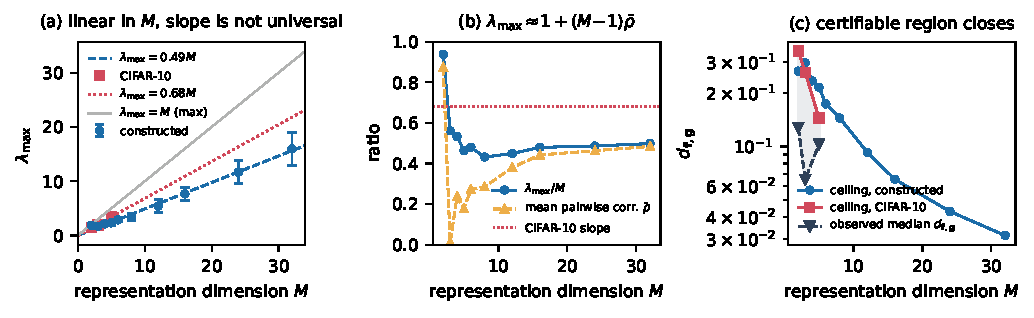
\includegraphics[width=0.92\textwidth]{fig_lamscale.pdf}
\caption{\textbf{(a)} $\lambda_{\max}$ is linear in $M$ on constructed models
($R^{2}=0.993$ over $M=2$--$32$), but the slope is not universal: $0.49$
constructed against $0.68$ on CIFAR-10, both well below the maximum
$\lambda_{\max}=M$. \textbf{(b)} The slope \emph{is} the mean pairwise
correlation of the log-ratio coordinates: for an equicorrelated matrix
$\lambda_{\max}=1+(M-1)\bar\rho$, so $\lambda_{\max}/M\to\bar\rho$, and the two
curves converge. The coordinates $z_{1,l}$ share a common pivot term, which
induces the correlation. \textbf{(c)} The certifiable region
$\dfg<1/(2\lambda_{\max})$ therefore closes as $M$ grows; shading marks where
observed CIFAR-10 dissimilarity still fits beneath it.}
\label{fig:lamscale}
\end{figure*}

\paragraph{Why certification degrades with dimension.}
$\lambda_{\max}$ is the largest eigenvalue of $\mathrm{Corr}(z_{1})$, whose
trace is $M$, so $\lambda_{\max}\in[1,M]$. Measured over $M=2$--$32$ on
constructed models it is linear in $M$ with $R^{2}=0.993$, and the slope equals
the mean pairwise correlation $\bar\rho$ of the log-ratio coordinates
(Fig.~\ref{fig:lamscale}): for an equicorrelated matrix
$\lambda_{\max}=1+(M-1)\bar\rho$. The correlation arises structurally, since
every coordinate $z_{1,l}=\log p(y_{l}|x)-\log p(y_{0}|x)$ shares the same
pivot term. The slope is setting-dependent --- $0.49$ on constructed models and $0.64$ on
CIFAR-10 over $M=2,3,5,8$ ($R^{2}=0.97$) --- so we report the formula rather
than a universal constant. Either way the ceiling $1/(2\lambda_{\max})$ falls
like $1/M$ and the method is a low-dimensional instrument.

\paragraph{Scope: language models.}
The family is motivated by autoregressive language modelling, where diversity
is easily met ($|\Y|\sim10^{4}$ against $M\sim10^{3}$) but confidence is
extreme --- only a few next tokens are ever plausible. Our results predict the
outcome there without running it. With
$\lambda_{\max}=1+(M-1)\bar\rho$ and $\bar\rho\in[0.49,0.68]$ across the two
settings we measure, the Prop.~\ref{prop:ceiling} ceiling at $M=64$ lies
between $0.011$ and $0.016$, far below any plausible $\dfg$ between retrained
models, while $\delta_{M+1}$ can only be worse than the $10^{-15}$ we measure
at $M=2$. Thm.~\ref{thm:maxdiv} should therefore certify nothing at that scale
and $\dKL$ should carry no representational information --- a falsifiable
prediction rather than an evasion, and one our released code tests directly.
The quantity to check is $\bar\rho$ in a tied-embedding transformer: if it
falls outside $[0.49,0.68]$, the formula rather than the conclusion is what
needs revising.

\paragraph{A caveat on the worst case.}
Our constructions realise a worst case that training does not generically
produce: on trained models KL retains a visible association with $\dfg$ even
where Thm.~\ref{thm:klcond} guarantees nothing at all. The theory describes
what \emph{can} go wrong, and the diagnostic of Sec.~\ref{sec:diagnostic} says
when it is likely to.

%%%%%%%%%%%%%%%%%%%%%%%%%%%%%%%%%%%%%%%%%%%%%%%%%%%%%%%%%%%%%%%%%%%%%%%%%%%%%%%
\section{Related Work}
\label{sec:related}

\paragraph{Similarity measures and their invariances.}
Comparing representations means choosing what to be invariant to, and the
choice is contested: CCA \citep{hotelling1936} and its variants
\citep{raghu2017,morcos2018} admit any invertible linear map, CKA
\citep{kornblith2019} only orthogonal transformations and isotropic scaling,
shape metrics \citep{williams2021} the orthogonal case, while RSA
\citep{kriegeskorte2008} compares similarity matrices. \citet{klabunde2025}
survey the field and observe that functional and representational measures need
not correlate. Recent empirical work sharpens this: the scaling trends read as
evidence for the Platonic Representation Hypothesis \citep{huh2024} are
confounded by width and depth, with alignment largely vanishing under
permutation-based null calibration \citep{aristotelian2026}; cross-modal
convergence degrades as evaluation sets grow \citep{platoscave2026}; and what
survives appears to be neighbourhood structure rather than metric geometry
\citep{structure2026}. Our width finding is consistent with this line, but
differs in method: our invariance class is fixed by identifiability rather than
chosen.

\paragraph{Functional similarity, and what it does not settle.}
A parallel line compares models by what their representations \emph{support}
rather than how they are shaped. Model stitching \citep{bansal2021} inserts a
trained affine map between one network's early layers and another's late ones
and asks whether performance survives, which tests whether representations are
interchangeable for the task. \citet{klabunde2025} document that functional and
representational measures need not agree, and \citet{sucholutsky2023} argue the
field lacks a shared vocabulary for what alignment should mean. Our question is
upstream of both: we ask what can be inferred about representations from the
\emph{output distribution alone}, without training a probe or a stitching
layer. That matters because output distributions are the one thing always
available --- from an API, from a checkpoint, from a published log --- and our
answer is that the inference is weaker than it looks, in a way that depends on
the divergence and on how confident the models are.

\paragraph{Identifiability, exact and approximate.}
The softmax family is identifiable up to invertible linear maps under
diversity, shown for conditional energy-based models
\citep{khemakhem2020icebeem}, the discriminative formulation
\citep{roeder2021} and the multi-task setting \citep{lachapelle2023}.
\citet{marconato2025} lift diversity, characterising distribution-equivalent
next-token predictors up to an extended-linear relation and obtaining an ``all
or none'' dichotomy structurally analogous to our Thm.~\ref{thm:dichotomy},
though theirs concerns which properties transfer and ours when a divergence can
detect non-equivalence. \citet{liu2026} prove next-token representations are a
linear transformation of latent posterior log-probabilities up to an
$o(\epsilon)$ term. What this literature supplies is the relation $\simL$; what
it does not supply is any statement about approximate agreement.

\paragraph{Robustness under approximate likelihood maximisation.}
\citet{reizinger2024} introduce $\varepsilon$-non-identifiability and
separately show cross-entropy can invert the data-generating process
\citep{reizinger2025}. \citet{buchholz2024} give the first robustness result
for nonlinear ICA under misspecification and note that not every identifiability
result survives slight misspecification --- the observation we make
quantitative here. \citet{nelson2026} distinguish statistical from structural
near-identifiability. Related failures are known for correlated factors
\citep{trauble2021} and independent mechanism analysis \citep{sliwa2022}.
Closest to us, \citet{nielsen2025} prove small KL does not guarantee
representational similarity; we take that as the boundary case $\alpha=1$,
extend it to every $\alpha\le1$, and supply the missing other side.

\paragraph{R\'enyi order as a dial on worst-case ratios.}
The family and its monotonicity are classical \citep{vanerven2014}, and its
extremes are exactly the regimes we contrast. Differential privacy turns on the
same distinction: $\varepsilon$-DP \emph{is} a max-divergence bound, and
R\'enyi DP \citep{mironov2017} interpolates between it and weaker average-case
guarantees. The trade-off recurs in variational inference, where the R\'enyi
bound interpolates between mode-seeking and mass-covering
\citep{li2016}, motivates tail-adaptive alternatives under heavy-tailed density
ratios \citep{wang2018} and admits monotonic schemes \citep{daudel2023}; and in
PAC-Bayes, where R\'enyi bounds replace the KL term \citep{begin2016}. In each
case the order governs how much weight the rarest events receive. We show
representational identifiability belongs in the same taxonomy, and locate its
threshold.

%%%%%%%%%%%%%%%%%%%%%%%%%%%%%%%%%%%%%%%%%%%%%%%%%%%%%%%%%%%%%%%%%%%%%%%%%%%%%%%
\section{Discussion and Conclusion}
\label{sec:discussion}

\paragraph{Limitations.}
\emph{(a)} Two of three positive results remain out of reach:
Thm.~\ref{thm:klcond} needs $\epsilon<1.7\times10^{-3}$ at best and
Cor.~\ref{cor:ceiling} needs $\alpha\approx64$ on our models against a
threshold near $1.35$. Thm.~\ref{thm:maxdiv} does certify, but the
$\dfg<1/(2\lambda_{\max})$ ceiling bounds its reach and the residual slack lies
entirely in passing from log-ratio perturbations to coordinate correlations.
Thm.~\ref{thm:graded} is valid on every trained pair we tested but exceeds the
realised $\dfg$ by two to three orders of magnitude, so it is a structural
statement rather than a usable bound.
\emph{(b)} Effect sizes here are small relative to seed noise. The temperature
effect is $+0.109$ and needed $30$ seeds to separate from zero; the dimensional
comparison rests on $10$ seeds per dimension and its intervals are
correspondingly wide. Conclusions from pair-level $p$-values in this setting
would be badly anticonservative, since $n$ seeds give $\binom{n}{2}$ dependent
pairs.
\emph{(c)} The worst case is not the typical case: KL retains substantial
empirical association with $\dfg$ on trained models even where our bounds say
nothing. \emph{(d)} Control is proved for embeddings and unembeddings, not
intermediate layers; $\dfg$ has a specific invariance class we do not claim is
the right one; diversity binds when classes are fewer than representation
dimensions. \emph{(e)} Our width result varies hidden width at fixed $M$ and
fixed dataset size, and the synthetic arm applies the accuracy filter of
\citet{roeder2021} only at analysis time. \emph{(f)} We predict rather than measure behaviour on language models
(Sec.~\ref{sec:exp}).

\paragraph{In practice.}
Three recommendations, all cheap. \emph{Report $\delta_{M+1}$ beside any
KL-based similarity claim.} It bounds in advance what that comparison can
reveal, and on a CIFAR-10 classifier it is $10^{-15}$ --- which is to say
nothing, however small the measured divergence. \emph{Prefer orders
$\alpha>1$ to KL when comparing confident models.} No order at or below $1$
controls (Cor.~\ref{cor:below}), and empirically KL's association with $\dfg$
collapses with representation dimension (Tab.~\ref{tab:c3}). \emph{Read
$\lambda_{\max}$ before trusting a perturbation-style guarantee.} It fixes the
largest dissimilarity the method could ever rule out, and grows with the
representation dimension, so a certificate that works at $M=2$ may be
structurally unavailable at $M=16$. More broadly, matched loss is not evidence
of matched representations, and the gap widens precisely as models become more
confident and their representations wider --- the regimes the field is moving
toward.

\paragraph{Conclusion.}
The representational error is an unweighted spread of log-likelihood ratios;
divergences weight labels by mass; the R\'enyi order measures the gap. Below
$\alpha=1$ nothing controls, above it every genuinely distinct pair is
eventually visible, and the interval between is closed by a computable
constant. The known failure of KL is the boundary case of this statement rather
than an isolated counterexample. What that buys in practice is narrower than
one would like: two of our guarantees cannot bite for reasons we can prove, and
the third certifies a majority of retrained CIFAR-10 pairs only at low
representation dimension. Where certification is out of reach, four quantities
computable in one forward pass still bound what a likelihood comparison could
reveal. Two findings emerged that we did not seek --- wider networks learning
closer distributions and further-apart representations, and both failure modes
tightening with dimension --- and the second says the regime where this theory
is usable is not the regime the field is moving toward. Closing that gap is the
natural continuation.

\section*{Impact Statement}
This is foundational work on when representation comparisons are meaningful.
The main societal relevance is that overclaiming representational agreement
from likelihood agreement can mislead interpretability and distillation
pipelines.

\bibliographystyle{plainnat}
\bibliography{references}

%% ===================== APPENDICES =====================
\newpage
\appendix
\onecolumn

\section{Notation}
\label{app:notation}

\begin{center}\small
\begin{tabular}{@{}ll@{}}
\toprule
symbol & meaning \\
\midrule
$\bff,\bfg$ & embedding $\X\to\mathbb{R}^{M}$ and unembedding $\Y\to\mathbb{R}^{M}$ \\
$\bff_{0},\bfg_{0}$ & displaced maps $\bff(x)-\bff(x_{0})$, $\bfg(y)-\bfg(y_{0})$ \\
$\bfL,\bfN$ & matrices with columns $\bfg_{0}(y_{i})$, $\bff_{0}(x_{i})$, $i=1..M$ \\
$\simL$ & linear equivalence: $\bff=\mathbf{A}\bff'$, $\bfg_{0}=\mathbf{A}^{-\top}\bfg'_{0}$ \\
$r_{y}(x)$ & log-ratio $\log p(y|x)-\log p'(y|x)$ \\
$R_{y}(x)$ & logit difference $\bff(x)^{\top}\bfg(y)-\bff'(x)^{\top}\bfg'(y)$ \\
$a_{y},b_{y}$ & margin gaps $s_{\hat y}-s_{y}$ and $s'_{\hat y}-s'_{y}$ \\
$E_{\alpha}(y)$ & tilted exponent $\alpha a_{y}+(1-\alpha)b_{y}$ \\
$\alpha^{\star}_{\mathrm{sym}}$ & $\min\{\alpha^{\star}(p\|p'),\alpha^{\star}(p'\|p)\}$ \\
$z_{1},z_{2}$ & $\bfL^{\top}\bff(x)$, $\bfL'^{\top}\bff'(x)$ \\
$\Delta_{l}$ & $z_{1,l}-z_{2,l}=r_{y_{l}}-r_{y_{0}}$ \\
$s_{l},s'_{l}$ & $\operatorname{std}_{x}(z_{1,l})$, $\operatorname{std}_{x}(z_{2,l})$ \\
$\mathrm{sd}_{l},\tau_{l},\psi_{l}$ & $\operatorname{std}(\Delta_{l})$, $|s_{l}-s'_{l}|$, $\min(s_{l},s'_{l})$ \\
$\lambda_{\max}$ & largest eigenvalue of $\mathrm{Corr}(z_{1})$; $\le M$ \\
$\delta_{m}$ & $\min_{x}\min_{y\in\Y_{m}}\min\{p(y|x),p'(y|x)\}$ \\
$\Delta$ & $\sup_{x,y}a_{y}(x)$ \\
\bottomrule
\end{tabular}
\end{center}

\section{Proofs for Section~\ref{sec:negative}}
\label{app:neg}

\subsection{Co-concentration (Lemma~\ref{lem:coconc})}

Along the norm-growth family the logits are $c\rho s_{y}$ with $s_{y}$ fixed,
so $p(y|x)=e^{-c\rho a_{y}}/Z_{\rho}$ with
$Z_{\rho}=1+\sum_{y\neq\hat y}e^{-c\rho a_{y}}$ and $a_{\hat y}=0$. Since
$a_{y}>0$ for $y\neq\hat y$, each summand vanishes and $Z_{\rho}\to1$, giving
$p(\hat y|x)\to1$. The angle-matching assumption gives the same $\hat y$ and
the same limit for $p'$, hence
$\|p-p'\|_{\TV}\to0$. Meanwhile
$|r_{y}|=c\rho|b_{y}-a_{y}|+O(1)=\Theta(\rho)$ whenever $a_{y}\neq b_{y}$.
\qed

\subsection{Rate lemma and critical order (Theorem~\ref{thm:alphastar})}

\paragraph{Set-up.}
For $\alpha\notin\{0,1\}$,
$\Dalpha=\frac{1}{\alpha-1}\log\sum_{y}p^{\alpha}p'^{1-\alpha}$. Substituting
$p\propto e^{-c\rho a_{y}}$, $p'\propto e^{-c\rho b_{y}}$,
\begin{equation}
\sum_{y}p^{\alpha}p'^{1-\alpha}
= Z_{\rho}^{-\alpha}Z_{\rho}'^{\,\alpha-1}
  \Big[1+\sum_{y\neq\hat y}e^{-c\rho E_{\alpha}(y)}\Big],
\qquad E_{\alpha}(y)=b_{y}+\alpha(a_{y}-b_{y}).
\label{eq:app-sum}
\end{equation}

\paragraph{(i) Decay below threshold.}
Expanding the three logarithms in \eqref{eq:app-sum} to first order,
\[
\log\textstyle\sum_{y}p^{\alpha}p'^{1-\alpha}
=\sum_{y\neq\hat y}\Big[e^{-c\rho E_{\alpha}(y)}
  -\alpha e^{-c\rho a_{y}}+(\alpha-1)e^{-c\rho b_{y}}\Big]+o(\cdot).
\]
Group the exponents $\{E_{\alpha}(y)\}\cup\{a_{y}\}\cup\{b_{y}\}$ by value; at
value $v$ the total coefficient is
$\#\{E_{\alpha}=v\}-\alpha\,\#\{a=v\}+(\alpha-1)\,\#\{b=v\}$. A label with
$a_{y}=b_{y}$ satisfies $E_{\alpha}(y)=a_{y}=b_{y}$ and contributes
$1-\alpha+(\alpha-1)=0$: such labels cancel exactly and must be excluded.
The decay rate $\kappa(\alpha)$ is the smallest $v>0$ with non-vanishing total
coefficient, giving $\Dalpha=\Theta(e^{-c\rho\kappa(\alpha)})$.

\paragraph{(ii) The case $\alpha=1$.}
At $\alpha=1$ we have $E_{1}(y)=a_{y}$, so every first-order coefficient
vanishes and the expansion above is uninformative. Computing directly,
\[
\dKL=\sum_{y}p\,(\log p-\log p')
   = c\rho\sum_{y\neq\hat y}(b_{y}-a_{y})e^{-c\rho a_{y}}/Z_{\rho}
     +\log(Z'_{\rho}/Z_{\rho}),
\]
whose leading term is $\Theta(\rho\,e^{-c\rho\min_{\mathcal{P}}a_{y}})$ with
$\mathcal{P}=\{y: a_{y}\neq b_{y}\}$. The polynomial prefactor is the signature
of the first-order cancellation.

\paragraph{(iii) Growth above threshold.}
If $E_{\alpha}(y)<0$ for some $y$ the bracket in \eqref{eq:app-sum} diverges
like $e^{c\rho\max_{y}(-E_{\alpha}(y))}$; dividing by $\alpha-1$ and taking the
logarithm gives growth that is \emph{linear} in $\rho$ with slope
$\max_{y}(-E_{\alpha}(y))/(\alpha-1)$. As $\alpha\to\infty$ this tends to
$\max_{y}(b_{y}-a_{y})$, which is $\Dinf/\rho$.

\paragraph{The threshold.}
$E_{\alpha}(y)$ is affine in $\alpha$ with $E_{0}(y)=b_{y}>0$. If
$a_{y}\ge b_{y}$ it is non-decreasing and never negative. If $a_{y}<b_{y}$ it
decreases and vanishes at $\alpha=b_{y}/(b_{y}-a_{y})$. Hence
$\alpha^{\star}=\min_{y:b_{y}>a_{y}}b_{y}/(b_{y}-a_{y})$, and since
$0<b_{y}-a_{y}<b_{y}$ we get $\alpha^{\star}>1$ unconditionally. \qed

\paragraph{Numerical verification.}
At a single input ($k=7$, $\rho\le160$) the bisected crossover matches
\eqref{eq:alphastar} to $2.8\times10^{-6}$ relative in the forward direction and
$1.2\times10^{-4}$ in the reverse; across $295$ geometries the median relative
error is $0.00\%$. Exponential rates match to $<2.3\%$ and linear slopes to
$<0.1\%$. Omitting the $a_{y}=b_{y}$ exclusion inflates predicted rates by
$40$--$70\%$. Code: \texttt{theory/perx.py}, \texttt{theory/rates.py}.

\subsection{Uniform separation (Theorem~\ref{thm:lower})}

Write $\bfL=\rho\,\mathbf{U}$, where the columns of $\mathbf{U}$ are the fixed
displaced unembedding directions, and likewise $\bfL'=\rho\,\mathbf{U}'$. The
measure $\dSVD$ standardises each coordinate of its arguments to unit variance
before forming the cross-covariance, so it is invariant to $z\mapsto cz$ for
any $c>0$. Hence
\[
\dSVD(\bfL^{\top}\bff,\ \bfL'^{\top}\bff')
=\dSVD(\mathbf{U}^{\top}\bff,\ \mathbf{U}'^{\top}\bff'),
\]
in which $\rho$ does not appear. Along the norm-growth family the embeddings
$\bff,\bff'$ are fixed by construction, so the right-hand side is a constant
$c$ of the geometry alone. By Thm.~\ref{thm:dichotomy}, $c=0$ if and only if
the pair is $\simL$-equivalent; the construction is not, so $c>0$. Therefore
$\max\dSVD\ge c>0$ uniformly in $\rho$. \qed

\paragraph{Numerical check.}
$\dSVD$ is constant to four decimals across $\rho\in\{1,5,20,80,320\}$ at every
geometry tested ($0.2123$, $0.4527$, $0.5996$ for permuted-cluster fractions
$q=0.25,0.5,0.75$ at $k=8$). Code: \texttt{theory/verify\_b3.py}.

\begin{remark}[A bound we do not claim]
One might hope for $c$ in closed form, for instance $c\ge q$ for the
permuted-cluster fraction $q$. That is false: across $28$ configurations
spanning $k\in\{4,8,12,20\}$ and $q\in[0.1,0.9]$ the inequality fails in $24$,
and none of $q$, $1-|1-2q|$, $2q(1-q)$ or $\min(2q,1)$ is a valid lower bound.
Measured $\dSVD$ ranges over $[0.05,0.86]$ and depends on the permutation
structure rather than on $q$ alone. Positivity is all the argument needs, and
Thm.~\ref{thm:dichotomy} supplies it.
\end{remark}

\section{Proofs for Section~\ref{sec:positive}}
\label{app:pos}

\subsection{Spectral step (Proposition~\ref{prop:tighten})}

Hoffman--Wielandt gives $\sum_{i}(\sigma_{i}-\tilde\sigma_{i})^{2}\le\|E\|_{F}^{2}$
for the singular values of $\Sigma_{z'z'}$ and $\Sigma_{z'w'}$. By
Cauchy--Schwarz, $\frac1M\sum_{i}|\sigma_{i}-\tilde\sigma_{i}|
\le(\frac1M\sum_{i}(\sigma_{i}-\tilde\sigma_{i})^{2})^{1/2}\le\|E\|_{F}/\sqrt{M}$.
This replaces the per-singular-value Weyl bound used previously and saves a
factor $\sqrt{M}$. \qed

\subsection{Perturbation bound (Theorem~\ref{thm:maxdiv})}

Write $\mu_{l}=\mathbb{E}[z_{1,l}]$. Since $z_{2,l}=z_{1,l}-\Delta_{l}$,
\[
z'_{l}-w'_{l}
=(z_{1,l}-\mu_{l})\Big(\tfrac1{s_{l}}-\tfrac1{s'_{l}}\Big)
+\frac{\Delta_{l}-\mathbb{E}\Delta_{l}}{s'_{l}}.
\]
The first term has standard deviation $|s'_{l}-s_{l}|/s'_{l}=\tau_{l}/s'_{l}$
and the second $\mathrm{sd}_{l}/s'_{l}$, so
$\operatorname{std}[z'_{l}-w'_{l}]\le(\tau_{l}+\mathrm{sd}_{l})/\psi_{l}$.

For the spectral step, $\|E\|_{F}^{2}=\sum_{j}\sum_{k}\Cov[z'_{k},\Delta'_{j}]^{2}$.
The inner sum is the squared norm of the projection of $\Delta'_{j}$ onto
$\mathrm{span}\{z'_{k}\}$ and is therefore at most
$\lambda_{\max}\Var[\Delta'_{j}]$, rather than the $M\Var[\Delta'_{j}]$ obtained
by applying the covariance inequality entrywise --- which would require all
$M^{2}$ entries to be simultaneously perfectly correlated. Combining with
Prop.~\ref{prop:tighten},
\[
\dSVD\le\frac{\|E\|_{F}}{\sqrt{M}}
\le\sqrt{\frac{\lambda_{\max}}{M}\sum_{l}\Var[z'_{l}-w'_{l}]}
=\sqrt{\lambda_{\max}}\,Q .
\]
The same argument on $\bfN^{\top}\bfg(y)$ bounds the unembedding term, and
$\dfg$ is their maximum. If $\Dinf\le\epsilon$ then
$|\Delta_{l}|\le2\epsilon$ pointwise, giving $\tau_{l},\mathrm{sd}_{l}\le2\epsilon$
and $Q\le4\epsilon/\psi_{\min}$. \qed

\paragraph{Why the two refinements matter.}
Aggregating coordinates in root mean square rather than taking the worst gains
$1.35$--$1.57\times$; keeping $\tau_{l}$ separate from $\mathrm{sd}_{l}$ gains a
further factor, since the difference of standard deviations is much smaller than
the standard deviation of the difference (median $\tau_{l}/\mathrm{sd}_{l}$ is
$0.25$--$0.53$). Jointly they tighten the bound by $1.65$--$2.37\times$, and on
CIFAR-10 by $1.67\times$: median bound $1.558\to0.931$, non-vacuity
$0\%\to58\%$, with $0/45$ violations.

\subsection{Non-vacuity ceiling (Proposition~\ref{prop:ceiling})}

In standardised coordinates $\Var[z'_{l}-w'_{l}]=2(1-\rho_{l})$ with
$\rho_{l}=(\Sigma_{z'w'})_{ll}$, so
$\sum_{l}\Var[z'_{l}-w'_{l}]=2M-2\operatorname{tr}(\Sigma_{z'w'})$. For any
square matrix the trace is at most the nuclear norm, and
$\sum_{i}\sigma_{i}=M(1-\dSVD)$, whence
$\sum_{l}\Var[z'_{l}-w'_{l}]\ge2M\dSVD$. Substituting into the bound of
Thm.~\ref{thm:maxdiv} gives $\mathrm{bound}\ge\sqrt{2\lambda_{\max}\dSVD}$, so
$\mathrm{bound}<1$ forces $\dSVD<1/(2\lambda_{\max})\le1/2$. \qed

\begin{remark}
The inequality $\sum_{l}\Var\ge2M\dSVD$ is identity-level, so the cap binds any
argument routed through a Frobenius-norm perturbation estimate. Escaping it
requires bounding the singular values of $\Sigma_{z'w'}$ directly. Empirically
the spectral form $\sqrt{2\lambda_{\max}(1-\bar\rho)}$ sits within $11$--$17\%$
of this floor, so essentially all residual looseness is in passing from
log-ratio perturbations to the correlations $\rho_{l}$.
\end{remark}

\subsection{KL on $\Thetadelta$ (Theorem~\ref{thm:klcond})}

For $y\in\Y_{m}$ and $p,p'\ge\delta_{m}$ there, the mean value theorem gives
$|r_{y}|=|\log(p_{y}/p'_{y})|\le|p_{y}-p'_{y}|/\delta_{m}\le\|p-p'\|_{1}/\delta_{m}$.
Pinsker gives $\|p-p'\|_{1}^{2}\le2D_{\mathrm{KL}}(p\|p')$, so
$\mathbb{E}_{x}[r_{y}^{2}]\le2\epsilon/\delta_{m}^{2}$ by Jensen. Then
$\rho_{2}\le2\max_{y}(\mathbb{E}_{x}r_{y}^{2})^{1/2}\le2\sqrt{2\epsilon}/\delta_{m}$,
and Thm.~\ref{thm:maxdiv} concludes. Only labels in
$\mathcal{Y}_{\mathrm{LLV}}\subseteq\Y_{m}$ enter $z_{1},z_{2}$, so the floor
need only be taken over $\Y_{m}$ and no tail-mass term appears. \qed

\begin{proposition}[The floor cannot be lifted]
\label{prop:floorcap}
For any model, $\delta_{M+1}\le1/(M+1)$, so \eqref{eq:klbound} is below $1$ only
for $\epsilon<1/(64(M+1)^{2})$; at $M=2$ this is $\epsilon<1.7\times10^{-3}$.
\end{proposition}
\begin{proof}
The $(M{+}1)$-th largest entry of a probability vector is at most $1/(M+1)$,
since $M+1$ entries each exceeding it would sum to more than one.
\end{proof}

\subsection{Dichotomy (Theorem~\ref{thm:dichotomy})}

$\alpha^{\star}(p\|p')=\infty$ means no $y$ has $b_{y}>a_{y}$, and
$\alpha^{\star}(p'\|p)=\infty$ means no $y$ has $a_{y}>b_{y}$; together
$a_{y}(x)=b_{y}(x)$ for all $x,y$. Since $a_{y}-b_{y}=R_{\hat y}-R_{y}$, this
says $R_{y}(x)=c(x)$ is independent of $y$, i.e.
$\bff(x)^{\top}\bfg(y)=\bff'(x)^{\top}\bfg'(y)+c(x)$. The additive $c(x)$
cancels in the softmax normaliser, so $p_{\bff,\bfg}=p_{\bff',\bfg'}$, and
linear identifiability gives $\simL$-equivalence under diversity. The converse
is immediate: equal distributions give $a_{y}=b_{y}$. \qed

\paragraph{Regression test.}
Over $329$ pairs, $\max|\dfg|=5.0\times10^{-4}$ in the $\infty$ class against
$\min|\dfg|=6.5\times10^{-2}$ in the finite class. The residual decays as
$O(1/n)$ in the sample size ($2.0\times10^{-3}$ at $n=500$,
$6.3\times10^{-5}$ at $n=16000$), the finite-sample bias of the
cross-covariance estimator; the CI tolerance is therefore $5/n$.

\subsection{Graded control (Theorem~\ref{thm:graded}) and the ceiling
(Corollary~\ref{cor:ceiling})}

If $\alpha^{\star}_{\mathrm{sym}}\ge A$ then $b_{y}-a_{y}\le b_{y}/A$ when
$b_{y}>a_{y}$ and $a_{y}-b_{y}\le a_{y}/A$ otherwise, so
$|a_{y}-b_{y}|\le\max(a_{y},b_{y})/A\le\Delta/A$. Since
$a_{y}-b_{y}=R_{\hat y}-R_{y}$, the map $y\mapsto R_{y}(x)$ lies within
$\Delta/A$ of the constant $R_{\hat y}(x)$, so its spread is at most
$2\Delta/A$ and $|\Delta_{l}|=|R_{y_{l}}-R_{y_{0}}|\le2\Delta/A$. Applying
Thm.~\ref{thm:maxdiv} gives $\dfg\le4\sqrt{M}\Delta/(\psi_{\min}A)$.
Inverting, for any $d_{0}>0$,
$\alpha_{0}(d_{0})=\sup\{\alpha^{\star}_{\mathrm{sym}}:\dfg\ge d_{0}\}
\le4\sqrt{M}\Delta/(\psi_{\min}d_{0})<\infty$. \qed

\section{Algorithms}
\label{app:alg}

\begin{algorithm}[H]
\caption{Representational dissimilarity $\dfg$}
\label{alg:dfg}
\SetAlgoLined
\KwIn{embeddings $\bff,\bff'$ on $N$ inputs; unembeddings $\bfg,\bfg'$;
      label subset with $|\Y_{m}|\ge M+1$; pivots $x_{0},y_{0}$}
\KwOut{$\dfg\in[0,1]$, zero iff the pair is $\simL$-equivalent}
$\bfL\leftarrow[\bfg_{0}(y_{1}),\dots,\bfg_{0}(y_{M})]$, $\bfL'$ likewise\;
$\bfN\leftarrow[\bff_{0}(x_{1}),\dots,\bff_{0}(x_{M})]$, $\bfN'$ likewise\;
$z_{1}\leftarrow\bfL^{\top}\bff(x)$, $z_{2}\leftarrow\bfL'^{\top}\bff'(x)$,
$w_{1}\leftarrow\bfN^{\top}\bfg(y)$, $w_{2}\leftarrow\bfN'^{\top}\bfg'(y)$\;
\ForEach{$(u,v)\in\{(z_{1},z_{2}),(w_{1},w_{2})\}$}{
  standardise each coordinate to zero mean, unit variance\;
  $\Sigma\leftarrow\mathrm{Cov}(u',v')$;\quad
  $d\leftarrow1-\frac1M\sum_{i}\sigma_{i}(\Sigma)$\;}
\Return $\max$ of the two values\;
\end{algorithm}



\section{Experimental Details}
\label{app:exp}

\paragraph{Constructed models.}
Unembeddings on a circle of radius $\rho$ (or quasi-uniform on $S^{M-1}$ for
$M\ge3$), embeddings sampled so each lies angularly nearest its own label. The
second model permutes unembedding \emph{directions} while keeping norms attached
to label indices, which preserves the top logit exactly; both models are
required to share the argmax, and the retained fraction is reported.

\paragraph{Synthetic.}
$20{,}000$ points from a $2$D Gaussian ($\sigma=3$), $c$ opposite-slice classes.
Embedding net: three LeakyReLU layers $2\to w\to w\to w\to 2$; unembedding: a
free $c\times2$ table. Adam, batch $128$, $15{,}000$ steps, $20$ seeds per cell,
$190$ pairs per cell, $3{,}800$ total.

\paragraph{CIFAR-10.}
ResNet18 embedding with an $M$-dimensional output; unembedding net of three
$128$-wide LeakyReLU layers followed by a linear map to $\mathbb{R}^{M}$. Adam,
batch $32$, $20{,}000$ steps, $10$ seeds. $45$ pairs per dimension; $270$ pairs
across dimensions and smoothing levels.

\paragraph{Statistics.}
Rank correlations are reported with $95\%$ cluster bootstrap intervals over
\emph{seeds} rather than pairs: $n$ seeds give $\binom{n}{2}$ dependent pairs,
so pair-level resampling is anticonservative. Point estimates elsewhere are
medians over pairs; App.~\ref{app:exp} gives the procedure.

\paragraph{Reproducibility guards.}
The analysis reports, never silently drops: the count of dropped pairs (must be
zero or be explained), the per-pair argmax agreement, and the assertion
$\alpha^{\star}_{\mathrm{sym}}=\infty\Rightarrow\dfg<5/n$. Three substantive
errors during this project were silent filters; the released CI suite guards
acceptance rate, the $5/n$ rule, the rate lemma in both directions, and the
proved constants.

\section{Additional Results}
\label{app:extra}

\paragraph{Tail localisation.}
Restricting both models to the reference model's top-$k$ support recovers
$44\%$, $65\%$ and $89\%$ of the full KL at $k=2,3,5$ for $M{=}2$, rising to
$67\%$, $84\%$ and $95\%$ at $M{=}5$; the $k{=}1$ entry is identically zero by
construction. So on a ten-class problem KL is spread over roughly half the
labels rather than concentrated on the argmax --- weaker tail localisation than
one might expect.

\paragraph{Averaging over inputs.}
Decay remains exponential under averaging ($R^{2}=1.00$ against $0.91$ for a
power-law fit) but the rate is set by the minimum margin in the support,
falling from $0.193$ to $0.018$ when clusters touch the decision boundary.

\paragraph{$\alpha^{\star}_{\mathrm{sym}}$ across geometries.}
Exhaustively over all $720$ permutations at $k=6$: rotations give
$\alpha^{\star}_{\mathrm{sym}}=\infty$ and $\dfg=-0.000$; reflections $1.109$;
order-breaking $1.047$. No permutation gives both a large critical order and
large dissimilarity. Non-uniform norms do not change this, and the median is
flat across $2$--$8$ cyclic-order violations --- the obstruction at $M=2$ is
topological rather than metric. Randomised search over $M\in\{2,\dots,12\}$
reaches $1.34$ with medians near $1.00$.

\paragraph{Positive control.}
Every experiment above asks whether the theory \emph{detects} a difference.
Thm.~\ref{thm:dichotomy} also makes the converse claim, which we test directly:
applying a known invertible $\mathbf{A}$ to a trained model
($\bff\mapsto\mathbf{A}\bff$, $\bfg_{0}\mapsto\mathbf{A}^{-\top}\bfg_{0}$)
produces a pair that is $\simL$-equivalent by construction. Across eight
CIFAR-10 models with $\mathrm{cond}(\mathbf{A})\in[2.4,5.1]$, all three
predictions hold: $\alpha^{\star}_{\mathrm{sym}}=\infty$ in every case,
$\Dalpha$ vanishes to machine precision at $\alpha\in\{0.5,1,2,\infty\}$
($\max|\Dalpha|\le1.3\times10^{-14}$), and $\dfg=1.000\times10^{-4}$ ---
\emph{exactly} $1/n$ at $n=10{,}000$ test inputs. That last value is worth
noting: the residual on an equivalent pair is a deterministic estimator bias of
$1/n$, not sampling noise, which is why our regression tolerance of $5/n$
carries a fivefold margin. The same holds at $M{=}8$, where
$\mathrm{cond}(\mathbf{A})$ reached $1.6\times10^{3}$ without affecting any of
the three.

\paragraph{Negative controls.}
A pointwise trade-off between $\alpha^{\star}(x)$ and the signal
$\max_{y}(b_{y}-a_{y})$ holds at fixed $x$ ($r=-0.58$ over $531$ geometries)
but does \emph{not} survive averaging: over an input distribution the
correlation falls to $-0.16$, and input concentration moves
$\alpha^{\star}_{\mathrm{sym}}$ and $\dfg$ in the same direction. The
label-smoothing arm on CIFAR-10 is confounded, since smoothing costs accuracy
($0.737\to0.633$) and moves $\dfg$; its correlations are non-monotone and we
draw no conclusion from them.



\end{document}
